\label{bg/beowulf}
A Cluster is a independent group of computer nodes combined into an unified system through network and software systems that allows data to move between nodes\citep{Gropp:beowulf}.

There are two main usage of Cluster computing. One is performance and the other is fault-tolerance. Cluster computers can provide high performance through parallel computation. Such parallelism is achieve by coordinating many processors for single problem. Cluster computers can be used to address three main computational constraints: Realtime-constraints, Throughput and Memory limitation\citep{Gropp:beowulf}. The Cluster computing is dominating the HPC worldwide. The most recent[November, 2016] list of top performing Supercomputers shows that 86.4\% of the Top 500 Supercomputers are Clusters based \citep{Top500:cluster}. 

The Beowulf project defines Beowulf as scaleable performance clusters based on commodity hardware, on a private system network with open source software infrastructure\citep{Beowulf.org}. The main purpose of a Beowulf cluster is to achieve performance through parallel computations. This is accomplished by running programs across a number of nodes simultaneously and they may need to coordinate during program execution\citep{Gropp:beowulf}.

In 1994, first Beowulf cluster project was started as a experimental platform for parallel computing by Thomas Sterling, Donald Becker and their team at the NASA Goddard Space Flight center. Their aim was to build a low cost HPC(High Performance Computing) system for scientific computation with commodity hardware and open source software bundle. \citep{Gropp:beowulf}

\subsection{Architecture}
A Beowulf Cluster consists of one master node and one or more compute nodes connected by a System Area Network. Figure in \ref{fig:beowulf_arch} shows a basic Beowulf architecture. The compute nodes are connected through a private network. Master node can be connected to the external network if required\citep{Gropp:beowulf}. Beowulf differs from Cluster of Workstation(COW) for the fact that the entire system behave like a single machine. Only master node provides user interface. The compute nodes can be diskless or may contain small local storage. Jobs are initiated, scheduled and assigned by the master node.

\begin{figure}[!htb]
  \center
  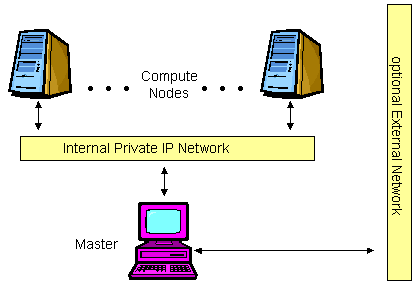
\includegraphics[width=.75 \linewidth]{figs/beowulf_arch.png}
  \caption{A basic Beowulf architecture. \citep{Beowulf:img}}
  \label{fig:beowulf_arch}
\end{figure}

\subsection{Hardware}
The main idea behind Beowulf project was to build HPC clusters using commodity hardware \citep{Gropp:beowulf}. The commodity hardware are those that are available Commercially-Off-The-Shelf (COTS) and not build for any specific purpose. These could be from PC-compatible hardware or rack-mounted servers to some embedded systems. The commodity status refers to the ability of obtaining such hardware on the open market and leveraging cheaper large scale productions. The biggest advantage of a Beowulf clusters is that it can be built with hardware produced by different vendors\citep{Thiru:05}

\subsection{Networking}
Beowulf clusters are group of individual machines that are meant to be interconnected to perform a task or number of tasks in parallel. In order to coordinate and complete execution efficiently the nodes in a cluster must be able to communicate with one another. Therefore, networks are very important components of a Beowulf cluster\citep{Gropp:beowulf}.

A Beowulf cluster with small number of nodes commodity networking technologies like Gigabit Ethernet are widely used. However, as the number of nodes increases network latency becomes a bottleneck for overall cluster performance. To overcome this, different network topology such hypercube topology and high-end networking hardware are used\citep{Thiru:05}.

\subsection{Software Infrastructure}
\paragraph{Operating Systems}
Linux is widely used on Beowulf clusters because it is open source, reliable and cost free. Another alternative is FreeBSD which is also open source. Open source nature of these Operating Systems are attractive to Beowulf community as it allows the kernel to be customised for specific needs and setup. \citep{Gropp:beowulf}

\paragraph{Middleware}
Coordination and communication between the processing nodes in cluster is key requirement. Beowulf utilises Message-passing model of parallel architecture. Both MPI and PVM(Parallel Virtual Machine) API can be deployed in a Beowulf systems. However, having a standard API and wider portability MPI become a popular choice for parallel programming in Beowulf. \citep{Gropp:beowulf}

\paragraph{Job control}
The Operating System only manages local jobs by itself. In distributed memory model additional job controller software is required. This job control program responsible for system partitioning, queuing jobs, how jobs start and run on remote nodes\citep{Gropp:beowulf}. Example of such parallel job control systems are PBS(Portable Batch System), Hydra and MPD. 